% !TeX root = ../paper_outline.tex

\begin{frame}{算法 1 | 两类工作流，一个统一的执行 DAG}
  \small
  任务分解型（Task-decomposition）与角色专门型（Role-specialized）描述不同的
  智能体生命周期和协作语义，但都转换为同一种按时间展开的带属性执行 DAG；
  两者不是互斥分类。

  \vspace{0.08cm}
  \begin{columns}[T,onlytextwidth]
    \begin{column}{0.48\textwidth}
      \centering
      \textbf{任务分解型：临时子智能体执行子任务}

      \vspace{0.05cm}
      \resizebox{0.92\linewidth}{!}{%
      \begin{tikzpicture}[
        n/.style={draw=AegisBlue,fill=AegisBlueLight,rounded corners=2pt,
                  minimum width=1.40cm,minimum height=0.68cm,align=center,font=\scriptsize},
        arr/.style={-{Stealth[length=1.6mm]},thick,draw=AegisGray}
      ]
        \node[n] (m0) at (0,0) {主智能体$^{(0)}$\\委派};
        \node[n] (a) at (2.2,1.05) {子任务 A};
        \node[n] (b) at (2.2,0) {子任务 B};
        \node[n] (c) at (2.2,-1.05) {子任务 C};
        \node[n] (m1) at (4.4,0) {主智能体$^{(1)}$\\汇合};
        \draw[arr] (m0) -- (a);
        \draw[arr] (m0) -- (b);
        \draw[arr] (m0) -- (c);
        \draw[arr] (a) -- (m1);
        \draw[arr] (b) -- (m1);
        \draw[arr] (c) -- (m1);
      \end{tikzpicture}
      }

      \scriptsize
      通常一次短生命周期调用对应一个节点；核心关系是
      \textbf{创建、扇出和汇合（spawn/fan-out/join）}。
    \end{column}
    \begin{column}{0.48\textwidth}
      \centering
      \textbf{角色专门型：持久角色跨阶段复用}

      \vspace{0.05cm}
      \resizebox{0.98\linewidth}{!}{%
      \begin{tikzpicture}[
        n/.style={draw=AegisOrange,fill=AegisOrangeLight,rounded corners=2pt,
                  minimum width=1.32cm,minimum height=0.68cm,align=center,font=\scriptsize},
        arr/.style={-{Stealth[length=1.6mm]},thick,draw=AegisGray}
      ]
        \node[n] (o0) at (0,0) {编排$^{(0)}$};
        \node[n] (r1) at (1.8,0) {研究$^{(1)}$};
        \node[n] (v1) at (3.6,0) {验证$^{(1)}$};
        \node[n] (r2) at (5.4,0) {研究$^{(2)}$};
        \node[n] (o1) at (7.2,0) {编排$^{(1)}$};
        \draw[arr] (o0) -- (r1);
        \draw[arr] (r1) -- (v1);
        \draw[arr] (v1) -- node[above,font=\tiny]{反馈} (r2);
        \draw[arr] (r2) -- (o1);
      \end{tikzpicture}
      }

      \scriptsize
      同一个研究者或编排者可对应多个节点；允许的反馈轮次
      在工作流启动前展开为固定激活片段。
    \end{column}
  \end{columns}

  \vspace{0.12cm}
  \begin{beamercolorbox}[rounded=true,sep=0.75ex,wd=0.98\textwidth]{block body}
    \scriptsize
    \textbf{统一映射：}节点是执行片段（execution episode），不是整个智能体；每个节点
    同时带有智能体、角色、子任务、激活轮次和请求属性。角色协议
    按 $R^{(1)}\!\rightarrow V^{(1)}\!\rightarrow R^{(2)}$ 预先展开，因此执行图固定且无环。
  \end{beamercolorbox}

  \vspace{0.06cm}
  \boundary{Real CC 轨迹直接验证 main/subagent 任务分解型工作流；固定轮次的
  角色专门型 DAG 是统一模型支持的输入形态，仍需带角色标注的轨迹单独验证。}
\end{frame}

\begin{frame}{算法 1 | 固定工作流 DAG 与剩余子图}
  \small
  工作流启动前已知完整 DAG；运行时只根据完成状态取其剩余诱导子图：
  \begin{equation}
    \begin{aligned}
      D_w&=(V_w,E_w),\\
      V_w^{\mathrm{rem}}(t)
        &=\{v\in V_w:\operatorname{status}_v(t)\neq\mathrm{completed}\},\\
      D_w^{\mathrm{rem}}(t)
        &=D_w[V_w^{\mathrm{rem}}(t)].
    \end{aligned}
    \label{eq:fixed-residual-dag}
  \end{equation}

  \scriptsize
  \renewcommand{\arraystretch}{1.14}
  \begin{tabularx}{\textwidth}{p{0.22\textwidth}X}
    \toprule
    规则 & 精确定义 \\
    \midrule
    工作流启动 & 任务/角色适配器在执行前生成全部节点、类型化边与固定轮次 \\
    边语义 & 每条 $e\in E_w$ 都是确定依赖，等价地取 $p_e=1$；不学习边概率 \\
    进度状态 & 节点只在待执行、执行中、已完成之间迁移，不新增分支、节点或边 \\
    剩余子图 & 已完成节点从式~\eqref{eq:fixed-residual-dag} 排除，其后继依赖随之释放 \\
    唯一不确定量 & 待执行或执行中片段的剩余时长 \\
    非研究范围 & 运行中才生成的新分支、无限反馈循环与随机拓扑 \\
    \bottomrule
  \end{tabularx}

  \vspace{0.08cm}
  \takeaway{当前算法 1 只解决“固定工作流拓扑 + 随机智能体执行片段时长”：
  拓扑序可以复用，进度或时间预测变化时重新运行 CPM。}
\end{frame}

\begin{frame}{算法 1 | 执行片段、类型化边与剩余时长}
  \small
  一个节点是固定 DAG 中的一次执行片段；同一智能体可以在不同
  子任务或角色阶段中对应多个节点。对未完成节点 $v$：
  \begin{equation}
    \begin{aligned}
      v&=\bigl(a_v,\rho_v,\tau_v,k_v,\mathcal R_v\bigr),\\
      e&=(u,v,\eta_e),\qquad
        \eta_e\in\{\mathrm{spawn},\mathrm{data},\mathrm{join},\mathrm{feedback}\},\\
      T_v^{\mathrm{rem}}(t)\mid\phi_v(t)&\sim F_v(t).
    \end{aligned}
    \label{eq:node-duration}
  \end{equation}

  \scriptsize
  \renewcommand{\arraystretch}{1.13}
  \begin{tabularx}{\textwidth}{p{0.20\textwidth}X}
    \toprule
    符号 & 含义与获得方式 \\
    \midrule
    $a_v$ & 智能体实例标识；持久角色的多个执行片段可共享同一 $a_v$ \\
    $\rho_v,\tau_v,k_v$ & 角色、子任务与激活轮次；用于区分两类工作流 \\
    $\mathcal R_v$ & 执行片段内的模型/工具请求；已完成轮次进入时间预测特征 \\
    $\eta_e$ & 固定因果边类型；反馈边通过预先定义的 $k_v$ 展开 \\
    $T_v^{\mathrm{rem}}$ & 从时刻 $t$ 到节点完成的随机剩余时长，单位为秒 \\
    $\phi_v(t)$ & 角色/类型、轮次数、已运行时间、词元数、API/工具延迟与负载 \\
    $F_v(t)$ & 条件时长分布；由 Quantile GBDT 的 P10/P50/P90 共同给出 \\
    \bottomrule
  \end{tabularx}

  \vspace{0.08cm}
  \takeaway{两类工作流只需要不同的工作流适配器；进入算法 1 后都成为
  类型化执行 DAG，后续 CPM 与松弛时间接口完全统一。}
\end{frame}

\begin{frame}{算法 1 | GBDT 输入特征与相关性}
  \small
  每个智能体完成一轮后，系统仅使用当时已经可见的信息构造
  $\phi_v(t)$，输入 GBDT 预测剩余执行时间：

  \vspace{0.03cm}
  \scriptsize
  \textbf{进度：}已完成轮次数、已运行时间；\quad
  \textbf{时延：}最近/平均 API 与工具/思考时长；\quad
  \textbf{词元：}最近/累计输入输出、历史最大输入；\quad
  \textbf{上下文：}角色、智能体类型、模型与请求类型。

  \vspace{0.03cm}
  \centering
  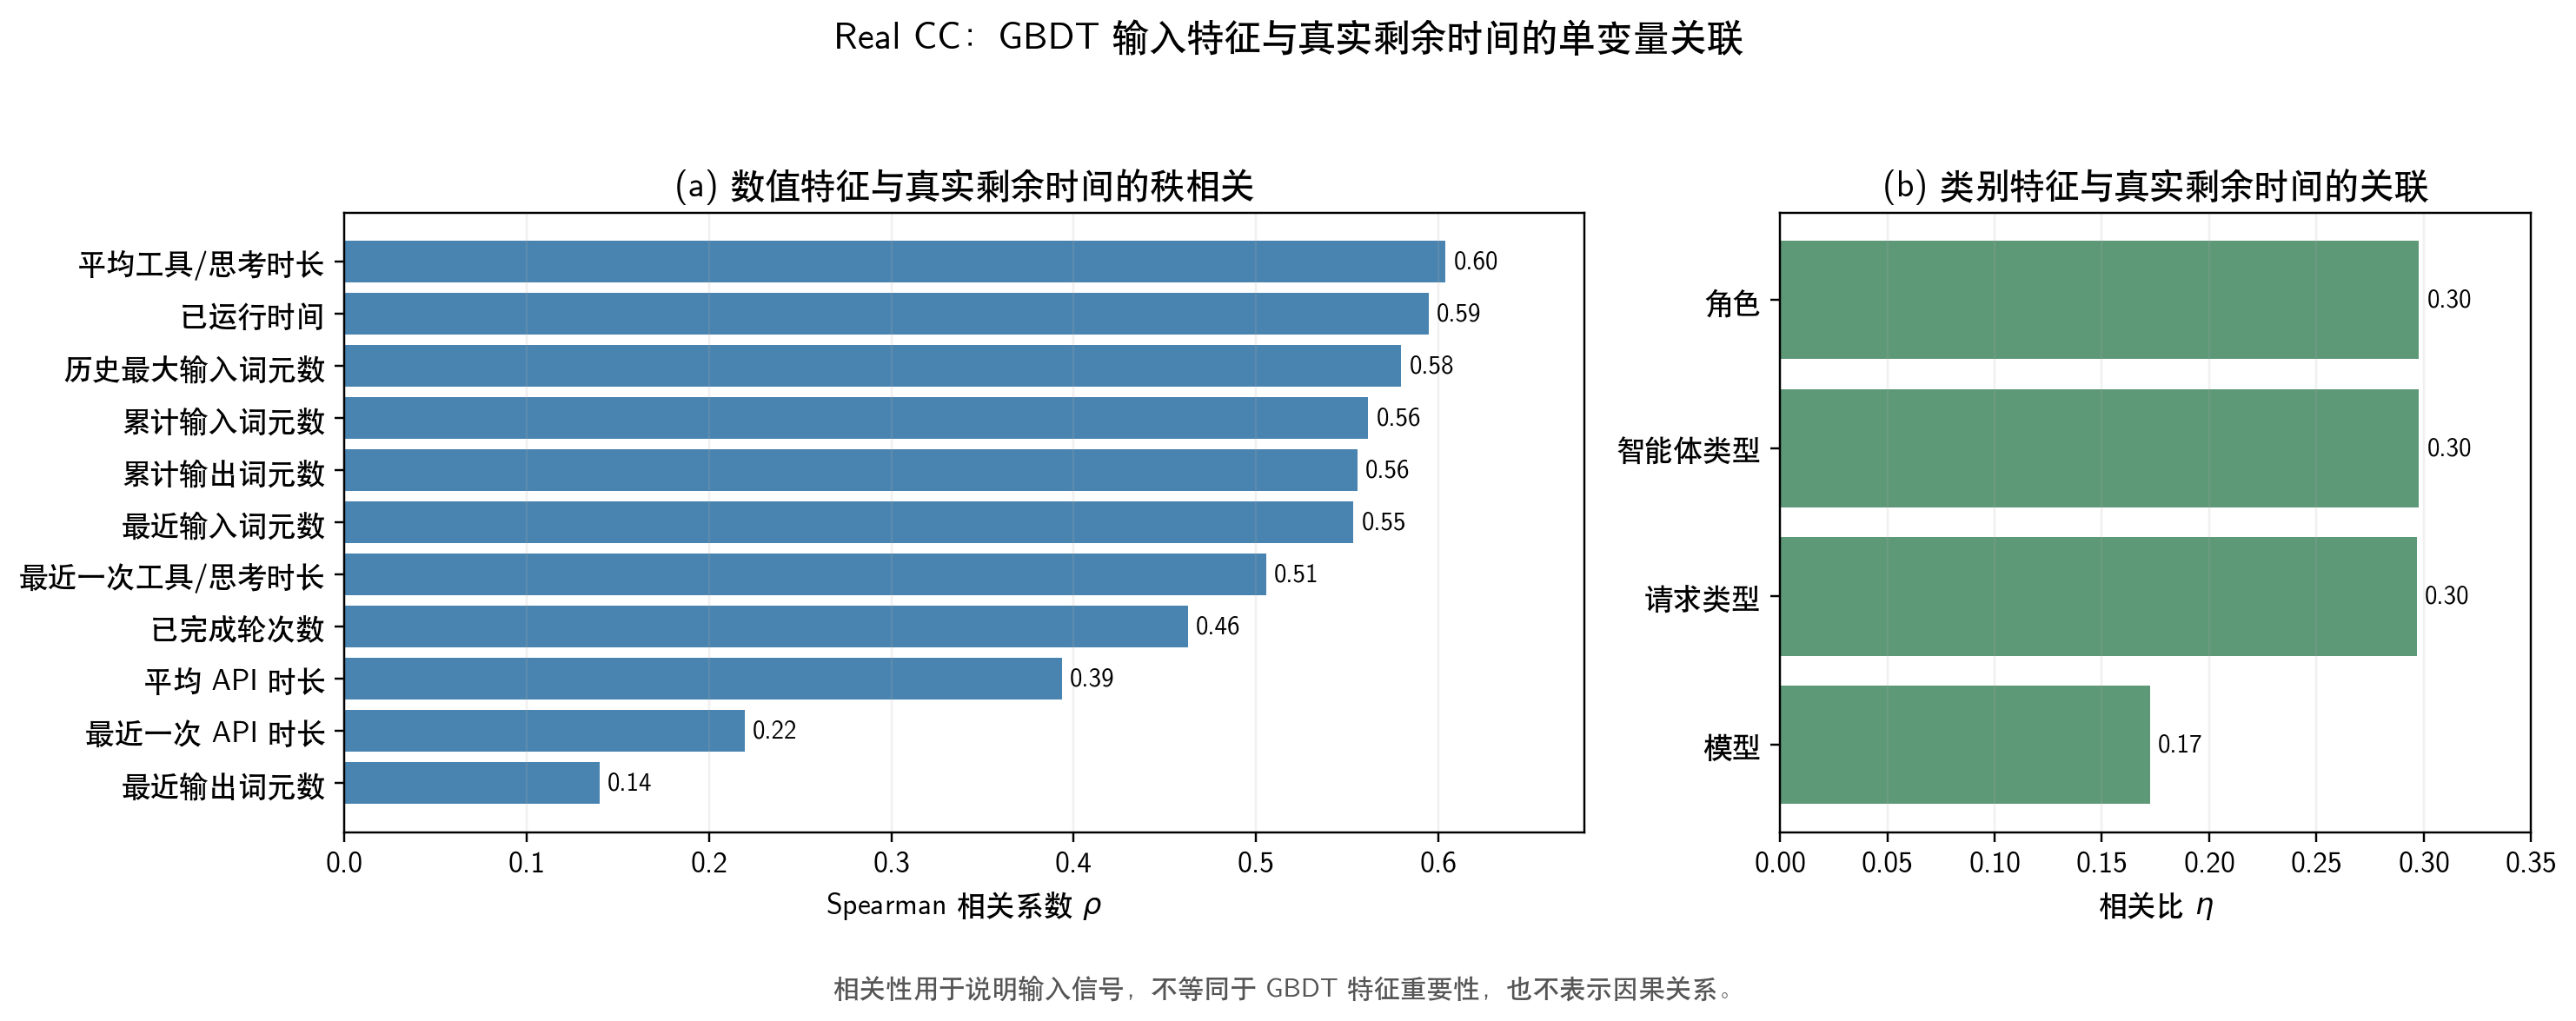
\includegraphics[width=0.99\linewidth,height=0.50\textheight,keepaspectratio]{fig_alg1_gbdt_feature_correlation.png}

  \vspace{0.02cm}
  \scriptsize
  图中数值特征使用 Spearman $\rho$，类别特征使用相关比 $\eta$；
  统计来自 393 个 Real CC 工作流的 96,103 个轮次结束样本。
  \takeaway{工具/思考时长、已运行时间和词元历史提供了最强的单变量信号；
  相关性只说明输入信号，不等同于 GBDT 特征重要性或因果关系。}
\end{frame}

\begin{frame}{算法 1 | GBDT 每轮更新后的预测准确度}
  \scriptsize
  GBDT 的模型参数在在线执行期间保持不变；每一轮结束后，系统更新
  $\phi_v(t)$ 并重新输出 P10/P50/P90，因而同一智能体的剩余时间预测
  会随新观测不断调整。下图以 P50 作为点预测。

  \vspace{0.02cm}
  \centering
  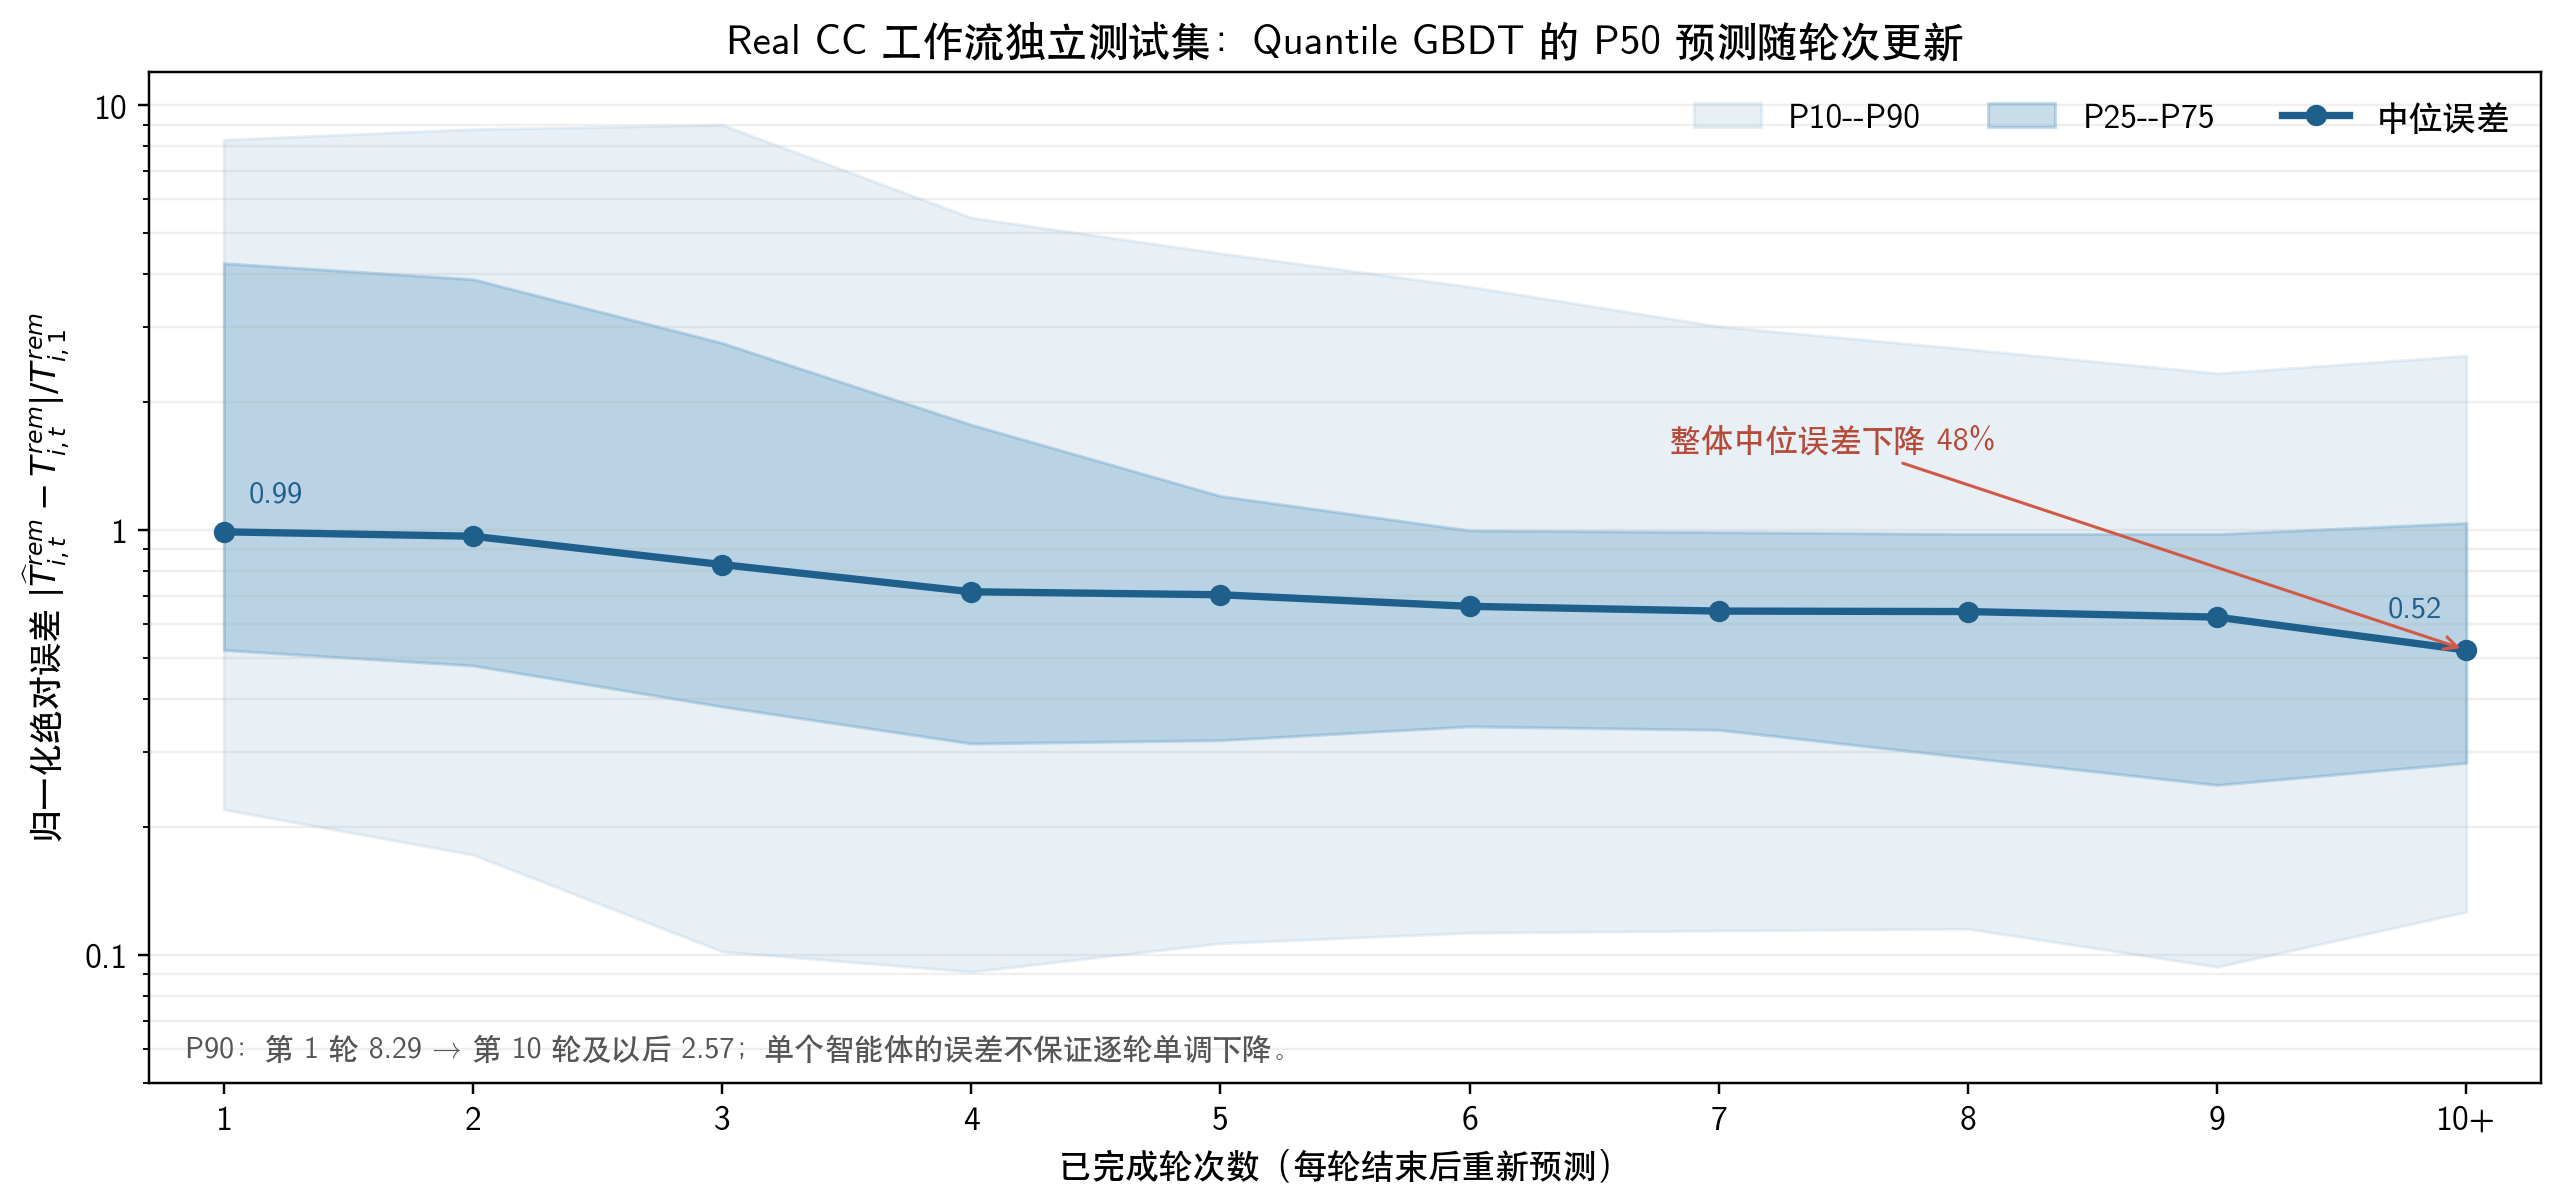
\includegraphics[width=0.99\linewidth,height=0.52\textheight,keepaspectratio]{fig_alg1_gbdt_accuracy_progress.png}

  \vspace{0.01cm}
  \scriptsize
  误差定义为
  $e_{i,t}=\lvert\widehat T_{i,t}^{\mathrm{rem}}-T_{i,t}^{\mathrm{rem}}\rvert/
  T_{i,1}^{\mathrm{rem}}$，使用每个智能体第一次预测时的真实剩余时间归一化。
  测试集包含 82 个与训练集工作流不重叠的工作流、17,074 个预测样本。
  \takeaway{总体中位误差由第 1 轮的 0.99 降至第 10 轮及以后的 0.52，
  P90 由 8.29 降至 2.57；总体准确度随信息积累改善，但单个智能体
  不保证逐轮单调改善。}
\end{frame}

\begin{frame}{算法 1 | CPM 入门：ES、EF、LS、LF 与 $S_v$}
  \small
  \textbf{CPM (Critical Path Method, 关键路径法)}：给定一个 DAG 和每个节点
  的执行时长，找出决定工作流完成时间的最长依赖路径，并计算每个
  节点在不拖慢工作流的前提下还能延迟多久。

  \vspace{0.08cm}
  \begin{columns}[T,onlytextwidth]
    \begin{column}{0.57\textwidth}
      \scriptsize
      \renewcommand{\arraystretch}{1.14}
      \begin{tabularx}{\linewidth}{p{0.13\linewidth}p{0.25\linewidth}X}
        \toprule
        符号 & 术语全称 & 直观含义 \\
        \midrule
        $ES_v$ & Earliest Start & 所有前驱完成后，$v$ 最早何时开始 \\
        $EF_v$ & Earliest Finish & 最早何时完成；$EF_v=ES_v+d_v$ \\
        $LS_v$ & Latest Start & 不增加 WCT 时，$v$ 最晚何时开始 \\
        $LF_v$ & Latest Finish & 不增加 WCT 时，$v$ 最晚何时完成 \\
        $S_v$ & Total Slack & 可吸收的额外延迟；
          $S_v=LS_v-ES_v=LF_v-EF_v$ \\
        \bottomrule
      \end{tabularx}
    \end{column}
    \begin{column}{0.40\textwidth}
      \centering
      \scriptsize
      \textbf{同一个节点的两种合法排程}

      \vspace{0.10cm}
      \begin{tikzpicture}[x=0.72cm,y=0.72cm,font=\tiny]
        \draw[-{Stealth[length=1.6mm]},draw=AegisGray] (0,0) -- (6.1,0)
          node[right] {$t$};
        \draw[fill=AegisBlueLight,draw=AegisBlue,thick]
          (0.7,1.05) rectangle (3.0,1.65);
        \node at (1.85,1.35) {时长 $d_v$};
        \node[below] at (0.7,1.05) {$ES_v$};
        \node[below] at (3.0,1.05) {$EF_v$};
        \node[left] at (0.4,1.35) {最早};

        \draw[fill=AegisOrangeLight,draw=AegisOrange,thick]
          (3.2,-0.05) rectangle (5.5,0.55);
        \node at (4.35,0.25) {时长 $d_v$};
        \node[below] at (3.2,-0.05) {$LS_v$};
        \node[below] at (5.5,-0.05) {$LF_v$};
        \node[left] at (2.9,0.25) {最晚};

        \draw[<->,draw=AegisGreen,thick]
          (0.7,2.0) -- (3.2,2.0)
          node[midway,above] {$S_v=LS_v-ES_v$};
        \draw[dashed,draw=AegisGreen] (0.7,1.7) -- (0.7,2.1);
        \draw[dashed,draw=AegisGreen] (3.2,0.65) -- (3.2,2.1);
      \end{tikzpicture}

      \vspace{0.08cm}
      \begin{beamercolorbox}[rounded=true,sep=0.75ex,wd=\linewidth]{block body}
        \scriptsize
        \textbf{前向计算：}计算 $ES/EF$ 与 WCT $L$。\par
        \textbf{后向计算：}从 $L$ 倒推 $LF/LS$。\par
        \textbf{关键节点：}$S_v=0$，不能再延迟。
      \end{beamercolorbox}
    \end{column}
  \end{columns}

  \vspace{0.06cm}
  \takeaway{松弛时间是节点的时间余量，不是执行时长；关键路径上的节点没有余量。}
\end{frame}

\begin{frame}{算法 1 | 前向计算：逐节点计算 $ES/EF$ 与 WCT}
  \small
  对式~\eqref{eq:fixed-residual-dag} 的一组时长实现值
  $\boldsymbol d^{(k)}=\{d_v^{(k)}\}$，按拓扑序从源节点向汇节点扫描：
  \begin{equation}
    ES_v^{(k)}
    =
    \max_{u\in\operatorname{pred}(v)}EF_u^{(k)},
    \qquad
    EF_v^{(k)}=ES_v^{(k)}+d_v^{(k)},
    \qquad
    L^{(k)}=\max_{z\in\operatorname{sink}}EF_z^{(k)}.
    \label{eq:cpm-forward}
  \end{equation}

  \scriptsize
  \centering
  \renewcommand{\arraystretch}{1.10}
  \begin{tabular}{lccccc}
    \toprule
    节点 $v$ & $d_v$ & 前驱节点 & $ES_v$ 的计算 & $ES_v$ & $EF_v$ \\
    \midrule
    Main & 3s  & --     & 源节点取 0         & 0  & 3  \\
    A    & 9s  & Main   & $EF_{\mathrm{Main}}$ & 3  & 12 \\
    B    & 6s  & Main   & $EF_{\mathrm{Main}}$ & 3  & 9  \\
    C    & 12s & Main   & $EF_{\mathrm{Main}}$ & 3  & 15 \\
    D    & 5s  & A, B   & $\max(12,9)$         & 12 & 17 \\
    E    & 6s  & B, C   & $\max(9,15)$         & 15 & 21 \\
    F    & 3s  & D, E   & $\max(17,21)$        & 21 & 24 \\
    \bottomrule
  \end{tabular}

  \vspace{0.10cm}
  \begin{columns}[T,onlytextwidth]
    \begin{column}{0.48\textwidth}
      \textbf{$ES_v$ 为什么取最大值？}\\
      $v$ 必须等待所有前驱节点完成，最晚完成的前驱决定其最早开始时间。
    \end{column}
    \begin{column}{0.48\textwidth}
      \textbf{工作流完成时间：}\\
      汇节点 F 的 $EF_F=24$s，因此本组实现值的剩余 WCT 为 $L=24$s。
    \end{column}
  \end{columns}
\end{frame}

\begin{frame}{算法 1 | 后向计算：计算 $LS/LF/S_v$ 与关键路径}
  \small
  令每个汇节点的 $LF=L$，再按逆拓扑序从汇节点向源节点扫描：
  \begin{equation}
    LF_v^{(k)}
    =
    \min_{z\in\operatorname{succ}(v)}LS_z^{(k)},
    \qquad
    LS_v^{(k)}=LF_v^{(k)}-d_v^{(k)},
    \qquad
    S_v^{(k)}
    =
    LS_v^{(k)}-ES_v^{(k)}
    =
    LF_v^{(k)}-EF_v^{(k)}.
    \label{eq:cpm-backward}
  \end{equation}

  \scriptsize
  \centering
  \renewcommand{\arraystretch}{1.08}
  \begin{tabularx}{0.94\textwidth}{lrrrrrX}
    \toprule
    节点 & $ES$ & $EF$ & $LS$ & $LF$ & $S_v$ & 解释 \\
    \midrule
    \textcolor{AegisRed}{\textbf{Main}} & 0  & 3  & 0  & 3  & \textbf{0} & 关键节点 \\
    A                                  & 3  & 12 & 7  & 16 & 4          & 可延迟至多 4s \\
    B                                  & 3  & 9  & 9  & 15 & 6          & 可延迟至多 6s \\
    \textcolor{AegisRed}{\textbf{C}}   & 3  & 15 & 3  & 15 & \textbf{0} & 关键节点 \\
    D                                  & 12 & 17 & 16 & 21 & 4          & 可延迟至多 4s \\
    \textcolor{AegisRed}{\textbf{E}}   & 15 & 21 & 15 & 21 & \textbf{0} & 关键节点 \\
    \textcolor{AegisRed}{\textbf{F}}   & 21 & 24 & 21 & 24 & \textbf{0} & 关键节点 \\
    \bottomrule
  \end{tabularx}

  \vspace{0.08cm}
  \begin{columns}[T,onlytextwidth]
    \begin{column}{0.48\textwidth}
      \textbf{$LF_v$ 为什么取最小值？}\\
      $v$ 必须赶在所有后继节点的 $LS$ 之前完成，最早的截止时间约束它。
    \end{column}
    \begin{column}{0.48\textwidth}
      \textbf{读表方法：}\\
      A 若额外延迟 4s，WCT 仍为 24s；C 若额外延迟 1s，WCT 就变为 25s。
    \end{column}
  \end{columns}

  \vspace{0.06cm}
  \takeaway{$S_v=0$ 的 Main $\rightarrow$ C $\rightarrow$ E $\rightarrow$ F 构成关键路径；
  一次 CPM 的复杂度为 $O(|V|+|E|)$。}
\end{frame}

\begin{frame}{算法 1 | 固定 DAG 松弛时间：只采样智能体剩余时间}
  \small
  固定式~\eqref{eq:fixed-residual-dag} 的拓扑，只从校准分布生成
  $K$ 组时长实现值，并分别运行 CPM：
  \begin{equation}
    d_v^{(k)}\sim F_v(t),
    \qquad
    \sigma_r^{(k)}(t)
    =
    S_{v(r)}\!\left(D_w^{\mathrm{rem}}(t),\boldsymbol d^{(k)}\right),
    \qquad
    \widehat\sigma_r(t)
    =
    Q_{q_\sigma}
    \!\left(
      \{\sigma_r^{(k)}(t)\}_{k=1}^{K}
    \right).
    \label{eq:request-slack}
  \end{equation}

  \begin{columns}[T,onlytextwidth]
    \begin{column}{0.47\textwidth}
      \scriptsize
      \textbf{固定拓扑}
      \begin{itemize}\tightitems
        \item 完整 $D_w$ 在工作流启动时已知；
        \item 所有边固定（等价 $p_e=1$），拓扑序可复用；
        \item 每组样本不改变节点或边；
        \item 节点完成只改变剩余节点集合。
      \end{itemize}
    \end{column}
    \begin{column}{0.50\textwidth}
      \scriptsize
      \textbf{唯一预测目标：智能体执行片段的剩余时间}
      \begin{itemize}\tightitems
        \item 用角色/类型、轮次数、已运行时间、词元数、
          工具/API 延迟与负载构造 $\phi_v(t)$；
        \item 预测器发布校准后的 $F_v(t)$，而不是单一点估计；
        \item 对每组 $\boldsymbol d^{(k)}$ 运行 CPM；
        \item $Q_{q_\sigma}$ 取低分位数，得到保守的请求松弛时间。
      \end{itemize}
    \end{column}
  \end{columns}

  \vspace{0.07cm}
  \boundary{拓扑不确定性不属于当前问题；动态分支或额外反馈轮次
  必须先编译成另一个固定 DAG，不能在一次工作流执行中改变图结构。}
\end{frame}

\begin{frame}{算法 1 | 在线过程与版本化输出}
  \begin{paperalgo}{算法 1：固定 DAG 工作流松弛时间估计}
    \algline{工作流启动前，用任务分解适配器或角色协议适配器构造固定 $D_w$，并发布不可变的 \code{dag\_version}。}
    \algline{根据轮次/节点进度更新待执行、执行中、已完成状态与式~\eqref{eq:fixed-residual-dag}。}
    \algline{按式~\eqref{eq:node-duration} 构造特征，并由 Quantile GBDT 更新 $F_v(t)$。}
    \algline{采样 $K$ 组智能体时长；每组用式~\eqref{eq:cpm-forward}--\eqref{eq:cpm-backward} 计算节点松弛时间。}
    \algline{按式~\eqref{eq:request-slack} 发布执行中请求的松弛时间分位数。}
    \algline{每次进度或时长模型更新只递增 \code{slack\_version}；\code{dag\_version} 保持不变。}
  \end{paperalgo}

  \vspace{0.06cm}
  \scriptsize
  \renewcommand{\arraystretch}{1.12}
  \begin{tabularx}{\textwidth}{p{0.20\textwidth}X}
    \toprule
    执行片段字段 & \code{workflow\_id}, \code{dag\_node\_id},
    \code{agent\_instance\_id}, \code{role}, \code{subtask\_id},
    \code{activation\_id}, \code{edge\_type}, \code{dag\_version} \\
    输出字段 &
    \code{predicted\_slack\_ms}, \code{slack\_quantile},
    \code{slack\_version} \\
    诊断字段 & \code{remaining\_p10/p50/p90}, \code{interval\_coverage},
    \code{prediction\_timestamp} \\
    过期策略 & 路由只接受单调不减的版本；超时快照按零松弛时间处理 \\
    \bottomrule
  \end{tabularx}
\end{frame}
